\documentclass{article}
\usepackage{amsmath, graphicx, amsfonts, caption, subfig, keyval}
\newcommand{\R}{\mathbb{R}}

\begin{document}
\title{Doing Things With Optimization (Working Title)}
\author{Jonathan Friedman \& Taylor Killiam}
\maketitle

%TODO before submission: make everything pretty and readable

\section{Introduction} \label{introduction}
Serving the maximum number of people at minimum expense is an important and general problem in industry. In this paper, we examine a subproblem of the case that arises when people receive service with quality proportional to their distance from a point of service. In particular, we study the problem of finding and placing the minimum number of points of service while still achieving a given level of service per person. Store placement provides an example of this rather general formulation. A person receives "service" proportional to their distance from a store, with people becoming increasingly unlikely to shop at a store as their distance from it increases. Thus, a company must balance placing their stores near as many people as possible with the cost associated with opening and maintaining a large number of stores.

This problem is easy to solve for one point of service. In section \ref{onepoint}, we give a solution for one point using compass search. However, compass search is not viable for a large number of points because the number of required directions to search grows at least quadratically(???). Instead, we use a clustering-based algorithm.
%TODO: Add more detailed explanation of what we're doing.

In section \ref{experiments}, we test our algorithm by optimizing placement of points of service in Massachusetts with population data from the U.S. 2010 Census \cite{census}.

\section{One Point of Service} \label{onepoint}
Compass search is a simple method of minimizing a function $f \in \R^n$. The gist of the algorithm is as follows (see \cite{survey} for details):

\begin{itemize}
  \item Choose $\lambda_1,...,\lambda_n$ to be a positive spanning set of $\R^n$. Also choose a starting guess $p_0$, a step size $s_0$, a scaling constant $\alpha<1$, and a tolerance $t$.
  \item For $k=0,1,...$:
  \begin{itemize}
    \item If $f(p_k + s_k\lambda_i) < f(p_k)$ for some $\lambda_i$, then set $p_{k+1} = p_k + s_k\lambda_i$ and set $s_{k+1} = s_k$.
    \item Otherwise, set $p_{k+1} = p_{k}$ and set $s_{k+1} = \alpha s_k$. If $s_{k+1} < t$, return $p_{k+1}$ as the minimum.
  \end{itemize}
\end{itemize}

In general, we minimize $$\sqrt{\sum_i f(\alpha_i) g(p, q_i)}$$ where $p$ is the location of the point of service, $\alpha_i$ and $q_i$ are the population at and location of point $i$, $h$ is the square root function, and the sum is over all points for which we have population data (in practice, because there are around 160,000 census blocks in Massachusetts, we subsample the population data to achieve better performance). Figure \ref{fig:popscale} shows point-of-service placement for various $f$, with $g(p-q_i) = ||p - q_i||^2$.

%TODO: make this figures actually readable by making point of service larger and removing key
\begin{figure}%
  \centering
  \subfloat[$f(\alpha_i)=\alpha_i$]{{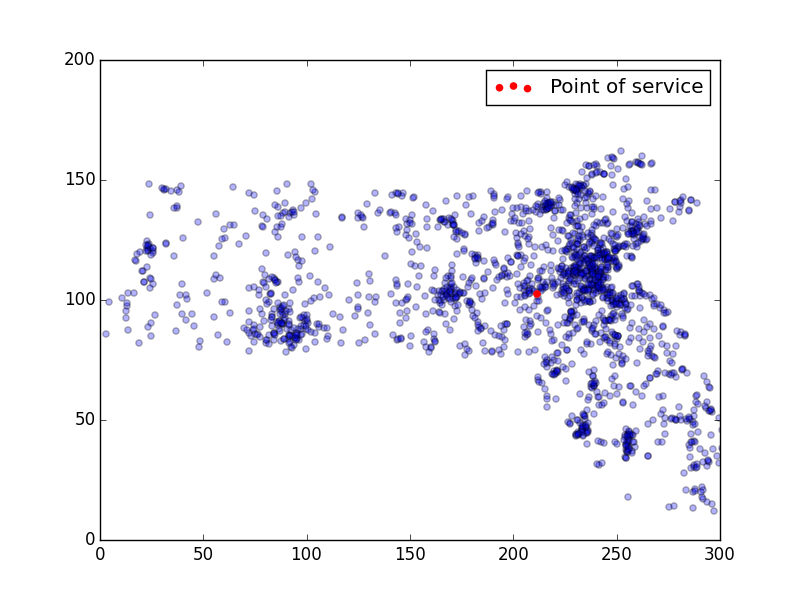
\includegraphics[width=5cm]{popscale.png} }}%
  \qquad
  \subfloat[$f(\alpha_i)=\sqrt{\alpha_i}$]{{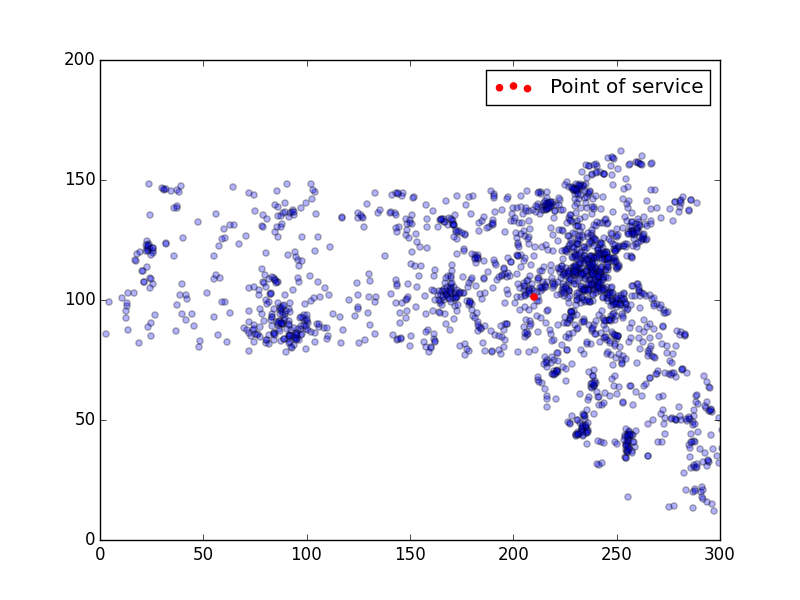
\includegraphics[width=5cm]{sqrtpopscale.png} }}%\\
  \qquad
  \subfloat[$f(\alpha_i)=\alpha_i^2$]{{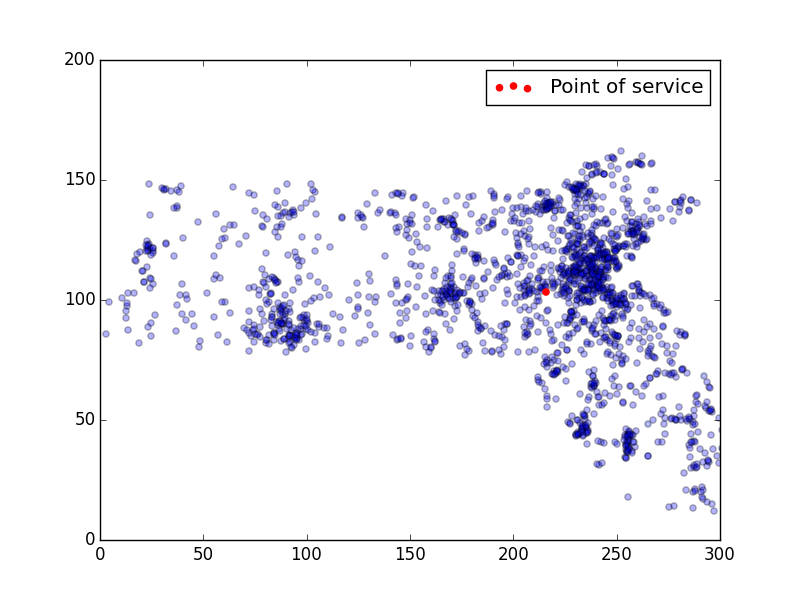
\includegraphics[width=5cm]{squarepopscale.png} }}%
  \qquad
  \subfloat[$f(\alpha_i)=\alpha_i^4$]{{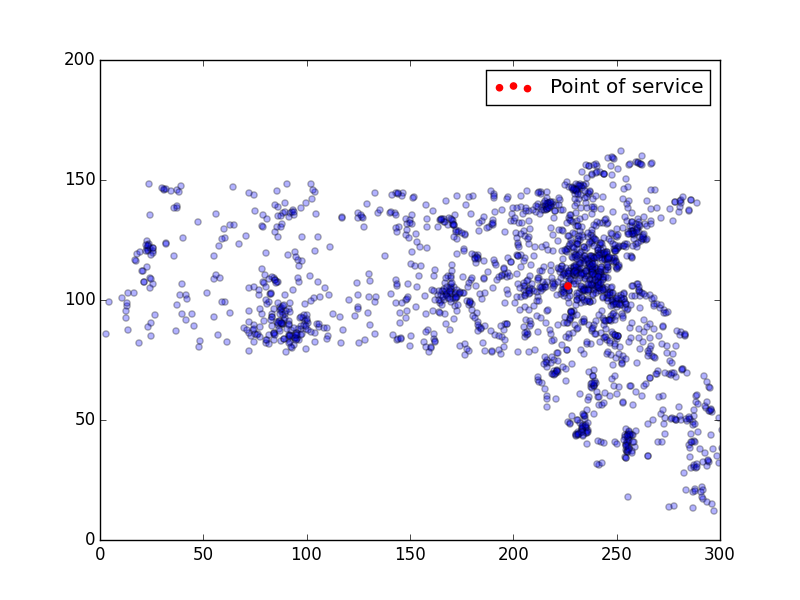
\includegraphics[width=5cm]{fourthpopscale.png} }}%
  \caption{Point-of-service placement under \\ various population scaling functions}
  \label{fig:popscale}
\end{figure}


This method works well for one point of service, but the number of directions to search grows at least quadratically with the number of points.  Consider the case of two points $p_1, p_2 \in \R^2$. Our function to minimize is now $$\sqrt{\sum_i f(\alpha_i)\min(g(p_1, q_i), g(p_2, q_i))}$$ which corresponds to minimizing each person's distance from the nearest point of service. A positive spanning set for $\R^n$ must contain at least $n+1$ vectors \cite{charles}, so we must consider at least 3 possible directions at each step for $p_1$ and $p_2$. For simplicity, consider the non-minimal positive spanning set of the four cardinal directions. IT IS BAD AND NOT GOOD SCALING.

% TODO: figure out how fast it actually scales
%The algorithm is then to find a direction for $p_1$ that produces a decrease, then find a direction for $p_2$ that produces a decrease. Even if the first possible direction evaluated for $p_1$, then the first possible direction for $p_2$, yield decreases,

\section{Experiments} \label{experiments}
%TODO: Describe we collected, parsed, subsampled, etc. census data.

\begin{thebibliography}{9}
  \bibitem{census}
  U.S. Census Bureau. \textit{TIGER/Line� with Selected Demographic and Economic Data: Population \& Housing Unit Counts}, 2010 Census. Nov. 9, 2015. https://www.census.gov/geo/maps-data/data/tiger-data.html.
  \bibitem{survey}
  Cite survey on optimization here
  \bibitem{charles}
  Cite "Theory of Positive Linear Dependence" here
\end{thebibliography}
\end{document}